\section{Metodologia}

Para concluir com êxito o desenvolvimento deste trabalho e consequentemente os 
objetivos propostos, o método utilizado para solução do problema é composto das 
seguintes etapas sequenciais:

\subsection{Coleta de textos}

Para as 
avaliações experimentais e análises realizadas neste estudo foram coletadas 
redações de um projeto organizado pelo Brasil Escola, que estimula o estudante 
a treinar a produção de textos do gênero dissertativo-argumentativo, sugerindo 
um tema, avaliando e publicando \cite{brasil_escola}. 

Nos dias atuais consegue-se facilmente coletar textos de páginas web, para esta 
tarefa, foi necessário criar um  \textit{crawler}. Existem diversas formas de 
implementar um \textit{crawler}, dentre elas, uma muito utilizada é o 
\textit{Scrapy}, utilizado neste trabalho \cite{scrapy}. O uso de um 
\textit{crawler}, permite explorar a estrutura de grafo da \textit{web}, 
navegar de uma página para outra identificando as \textit{tags} HTML que contém 
os dados necessários para compilar um \textit{dataset}. A figura 
\ref{figure:metodologia_1} ilustra a etapa em que o \textit{crawler} navega 
entre as páginas HTML, filtra as \textit{tags}, coleta e armazena os dados em 
um \textit{dataset}.

\begin{figure}[H]
\begin{center}
    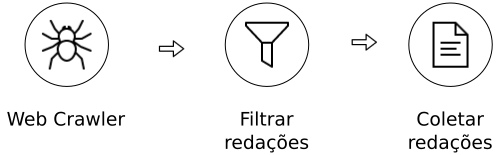
\includegraphics[scale=0.70]{images/metodologia_1.png}
\end{center}
\caption{O \textit{crawler}, navega entre as páginas HTML do banco de redações 
de forma metódica e automatizada indexando textos que posteriormente serão 
filtrados, coletados e armazenados.}
\label{figure:metodologia_1}
\end{figure}

\subsection{Pré-processamento, indução e testes}

A ferramenta de \textit{Data Mining} \textit{Orange} utilizada neste estudo 
permite o pré-processamento de dados, divisão do \textit{dataset} para 
treinamento e teste, bem como, a inferência simultanea dos classificadores 
\textit{Adaboost} e \textit{Naive Bayes}. O resultados das métricas de 
desempenho obtidos podem ser plotados para avaliação e comparação dos 
classificadores \cite{wahbeh2011comparison}.

A figura \ref{figure:metodologia_2} ilustra as etapas necessárias para 
pré-processamento, indução e testes dos algoritmos de Aprendizado de Máquina. 
Uma vez gerado o \textit{dataset} ná etapa anterior, no primeiro passo os 
documentos armazenados necessitam de um pré-processamento. Devido a sua 
natureza textual não estruturada, cada sentença do texto é separada em 
\textit{tokens} para transformar esses dados não estruturados em um formato 
estruturado, especificamente uma tabela atributo-valor denominada 
\textit{bag--of--words}. Nesta abordagem, palavras pouco significativas como 
artigos, preposições e conjunções que pouco caracterizam os texto podem ser 
ignoradas com uma ou mais listas de \textit{stopwords}. Segundo 
\cite{matsubara2003pretext}, este passo é importante, visto que a representação 
desses textos tem uma influência fundamental no resultado da indução dos 
algoritmos de Aprendizado de Máquina. No segundo passo é necessário definir os 
parâmetros de inferência de cada algoritmo e induzir os modelos classificadores 
\textit{Adaboost} e \textit{Naive Bayes}. O terceiro e último passo, o 
resultado da inferência dos classificadores são avaliados com as principais 
métricas de análise de classificadores citadas na literatura de Aprendizado de 
Máquina. Os passos dois e três são repetidos até que um do classificadores 
apresente resultados relevantes ao estudo.

\begin{figure}[H]
\begin{center}
    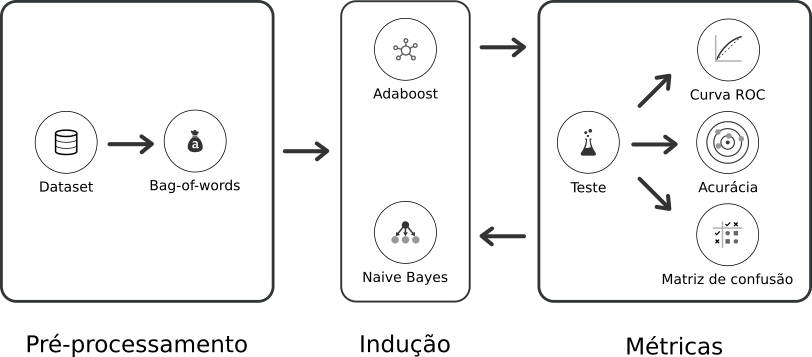
\includegraphics[scale=0.70]{images/metodologia_2.png}
\end{center}
\caption{O pré-processamento converte os texto em uma tabela }
\label{figure:metodologia_2}
\end{figure}